\chapter{Reinforcement Learning}
\label{chp:reinforcement-learning}


% %
% HEADER
% %
The nature of learning is strictly related with the process of learning by interacting with the environment.
Learning from interactions is a foundational idea underlying nearly all theories of learning and intelligence.
In fact, experimenting the consequences of actions allows to acquire knowledge about the environment and ourselves in order to achieve goals.

In this Chapter we introduce reinforcement learning, that is a computational approach to learning from goal-driven interactions with a dynamic environment.
%
In particular, we focus on $\mathcal{Q}$-learning, that is the most representative reinforcement learning technique.
%
For a more complete and general coverage of reinforcement learning, we refer the reader to \cite{sutton1998reinforcement}, \cite{szepesvari2010algorithms} and \cite{kaelbling1996reinforcement}.


% %
% MACHINE LEARNING BACKGROND
% %
\section{Machine Learning Background}
\label{sec:reinforcement-learning-machine-learning-background}

Machine learning is the field of artificial intelligence that gives computers the ability to learn without being explicitly programmed and to automatically improve learning and behavioral performance with experience.
%
To be more precise, as stated in \cite{mitchell2006discipline}, we say that a machine $M$ learns with respect to a particular task $T$, performance metric $P$, and type of experience $E$, if $M$ reliably improves its performance $P$ at task $T$, following experience $E$.

We do not want to provide an exhaustive coverage of the machine learning field, but giving the necessary background to better contextualize reinforcement learning as an attractive machine learning paradigm.
%
For a complete overview of machine learning, we refer the reader to \cite{samuel2000some}.

All machine learning tasks can be reduced to an archetypal machine learning task consisting of a learning agent (agent, for short) with the goal of inferring some functional relationship $F$ between inputs $i\in I$ and outputs $o\in O$.
%
We say that an input is \textit{labeled} if it is presented to the agent as a pair $(i,o).F(i)=o$, otherwise it is \textit{unlabeled}.
Furthermore, we say that an input is \textit{statically labeled} if $(i,o_{1}) \wedge (i,o_{2}) \Rightarrow o_{1}=o_{2}$, otherwise it is \textit{dynamically labeled}.

Machine learning tasks are traditionally classified into four broad categories: \textit{supervised learning}, \textit{unsupervised learning}, \textit{active learning} and \textit{reinforcement learning}.
%
Notice that in literature, both active and reinforcement learning are sometimes classified as special form of semi-supervised learning.
%
\textit{Supervised learning} consists of a learning agent that is presented with statically labeled inputs. The goal is to generalize the functional relationship so as to act correctly in situations not presented in the training set.
%
\textit{Unsupervised learning} consists of a learning agent that is presented with unlabeled inputs. The goal is to find patterns hidden in collections of unlabeled data.
%
\textit{Semi-supervised learning} consists of a learning agent that is presented with a minority of statically labeled inputs and a majority of unlabeled inputs.
%
\textit{Active learning} consists of a learning agent that queries the environment to obtain statically labeled inputs.
%
\textit{Reinforcement learning} consists of a learning agent that modifies the environment to obtain dynamically labeled inputs as a result of trial-and-error interaction with the environment.

In this work we focus on reinforcement learning because 
(i) it learns from the environment by modifying it and
(ii) it can benefit from prior knowledge about the environment, without assuming it.
%
All these aspects make reinforcement learning suitable for the realization of smart elasticity, that is elastic resource management leveraging machine learning.
%
Furthermore, other aspects that make reinforcement learning really exciting are that
(i) it fruitfully interacts with other scientific disciplines, such as statistics, optimization, psychology and neuroscience, 
(ii) that among all the forms of machine learning, it is the most closely inspired by biological learning systems, e.g. humans and animals, and
(iii) it leads the trend of artificial intelligence focused on learning driven by simple general principles


% %
% Reinforcement Learning Problem
% %
\section{Reinforcement Learning Problem}
\label{sec:reinforcement-learning-reinforcement-learning-problem}
Reinforcement learning is a machine learning paradigm focused on learning the best decision-making strategy to control a system from goal-driven interactions with an environment.
%
The reinforcement learning problem consists of an \textit{agent} determining the \textit{policy} to control a \textit{system} so as to maximize a the \textit{long-run value} of its behavior, through \textit{trial-and-error interactions} with the \textit{environment}.
%
In the following, we assume that the system to control and the environment to sense are the same, i.e. the agent learns how to control the system interacting with it.


The notions of \textit{trial-and-error interaction} and \textit{long-run value} are really important in reinforcement learning.
%
The concept of \textit{trial-and-error interaction} consists in the fact that each action taken by the agent on the system are immediately judged to be good or bad, accordingly to some rewarding mechanism.
%
The concept of \textit{long-run value} consists in the fact that the agent learns from delayed rewards, that is it may take a long sequence of actions, receiving insignificant reward, then finally arrive at a state with high reward.
%
Hence the agent must be able to learn which actions are desirable based on reward that can take place arbitrarily far in the future.

The standard reinforcement learning model is shown in Figure \ref{fig:reinforcement-learning-model}.
%
The environment communicates its own state $x$, from which the agent calculates 
(i) the perceived state $\tilde{x} = S(x)$, that is the portion of the state that the agent is interested in, and
(ii) the reward $r=R(x)$, that measures how good has been the last state transition, hence how good has been the last action taken.
%
The agent calculates the action $a=\pi(x)$ to be executed on the environment; the latter transits to a new state, in response to the taken action; and the cycle is repeated.
%
The agent's objective is to determine the policy that maximizes the \textit{total reward} achieved in the long-run.
%
In the following we assume that $S$ is the identity function, because the agent is interested in the environment state as a whole; hence we omit the $\tilde{x}$ notation and we will denote with $x$ the state perceived by the agent.
%The learning problems differ in the details of how the data is collected and how performance is measured.

\begin{figure}	
	\label{fig:reinforcement-learning-model}
	\centering
	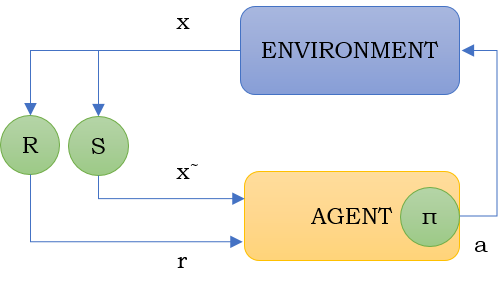
\includegraphics[width=.7\columnwidth]{reinforcement-learning-model}
	\caption{The standard reinforcement learning model.}
\end{figure}

The most important distinguishing characteristics of reinforcement learning are that
(i) it is a closed-loop problem\footnote{a \textit{closed-loop problem} is a problem that is solved iteratively and each iteration affects the input on the next one.},
(ii) it does not have wired instructions to decide a priori what actions to take in response to state transitions,
(iii) it does not rely on supervision nor on a complete model of the environment and
(iv) consequences of actions are perceived as to play out over extended time periods.

Reinforcement learning is of great interest because of the large number of practical applications that it can be used to address, ranging from problems in artificial intelligence to operations research or control engineering. In Section \ref{sec:reinforcement-learning-applications} we review a few of the most representative applications.

A reinforcement learning model is made of an \textit{environment}, an \textit{agent}, a \textit{policy}, a \textit{reward signal}, a \textit{value function} and an optional \textit{model} of the environment.

The \textit{environment (or controlled system)} is a dynamic, non-deterministic and stationary finite-state automaton.
It is a finite state automaton in the sense that at any given time it is fully characterized by its \textit{state}.
It is dynamic in the sense that it changes its own state in response to external stimulus.
It is non-deterministic in the sense that the same action taken on the same state in different instants may not produce the same state transition.
It is stationary in the sense that the probabilities of making state transitions do not change over time.

The \textit{agent} senses the state of the environment and takes \textit{actions} on the environment. The agent must be able to 
(i) sense the environment state,
(ii) take actions that affect it, 
(iii) chose actions driven by goals related to the environment state, and
(iv) use its experience to improve its performance over time.
%
At the same time, the agent cannot predict the effect of its actions on the environment; thus it has to monitor the environment frequently.

The \textit{reward signal (or reinforcement signal)} defines the short run convenience of taking a specific action in a given state.
Every time the agent takes an action on the environment, the latter changes its state and sends to the agent a reward representing the convenience of the action.
The reward signal thus defines what are the good and bad events for the agent.
Typically, it is realized by a stochastic function of the environment state and the actions taken.
If an action selected by the policy is followed by low reward, then the policy may be changed to select some other action in that situation in the future.
The agent objective is to maximize the total reward it receives over the long run.
The agent cannot alter directly the process that generates the reward signal, but can do it indirectly by changing the state of the environment through actions.

The \textit{value function} defines the long run convenience of a state, that is the total amount of reward an agent can expect to accumulate over the future, starting from that state.
To better understand the difference between rewards and values, notice that a state might always yield a low reward but still have a high value because it is regularly followed by other states that yield high rewards; and vice versa.
The goal of the agent is to determine a policy that maximize values, hence action choices rely on judgments about values rather than rewards.
However, there could be no values without rewards.
Determining values are much harder than rewards because the former must be continuously re-estimated from observations over time, whereas the latter are given given directly and immediately by the environment.
The value function is arguably the most important component in a reinforcement learning algorithm because an effective value function can make search in the space of policies more efficient.
Furthermore, the use of value function to discriminate policies distinguishes reinforcement learning from evolutionary methods that search directly in policy space driven by scalar evaluation of entire policies.

The \textit{policy} defines how the agent behaves in response to state changes of the environment.
Basically, it is a mapping from perceived states of the environment to actions to be taken when in those states.
It is typically realized by a simple stochastic function, whereas in some case it may involve extensive computation, such as a search process. 
An \textit{optimal policy} is the one that maximizes the long-run reward.

The \textit{model of the environment} defines the behavior of the environment, allowing to infer, given a state and an action, the resultant next state and next reward.
Models are used to consider possible future situations before they are actually experienced. For example, a model can be used by an agent to exclude a priori some actions with respect to others in a given state.
The main advantage of using models is the reduction of the exploration cost.
Reinforcement learning algorithms that leverage models are called \textit{model-based methods}, as opposed to simpler \textit{model-free methods} that are pure trial-and-error learners.

The comprehension of the difference between rewards and values is really important.
In literature, it is sometimes explained with analogies from the human domain, where the reward signal is somewhat like pleasure (if high) and pain (if low), whereas values correspond to a more refined and farsighted judgment of how pleased or displeased we are that our environment is in a particular state.


% %
% REINFORCEMENT LEARNING ALGORITHM
% %
\section{Reinforcement Learning Algorithm}
\label{sec:reinforcement-learning-algorith}
There are plenty of exact and heuristic techniques to solve the reinforcement learning problem.
Although they vary a lot, they share a common algorithmic structure, shown as pseudo-code in Algorithm \ref{alg:reinforcement-learning-general}.

\begin{algorithm}[t]
	\label{alg:reinforcement-learning-general}
	\SetKwInOut{Input}{input}
	\SetKwInOut{Input}{input}
	\SetKwInOut{Output}{output}
	
	\Input{state space $\mathcal{X}$, action space $\mathcal{A}$}
	
	\Output{none}
	
	initialize $V[X,A]$ \\
	observe current state $x$ \\
	\While{stop criterion $=$ False}{
		$a \leftarrow argmax_{a\in\mathcal{A}} V[x,a]$ \\
		carry out action $a$ \\
		observe new state $x'$ \\
		observe reward $r$ \\
		update $V[x,a]$ using $x'$ and $r$ \\
		$x \leftarrow x'$ \\
	}
	
	\caption{Pseudocode of the general reinforcement learning algorithm.}
\end{algorithm}

%Notice that, the set of admissible actions may differ from state to state. Given a state $x\in\mathcal{X}$, we denote with $\mathcal{A}_{x}\subseteq\mathcal{A}$ the subset of admissible actions for the state $x$.


\section{Experience and history}
\label{sec:reinforcement-learning-experience-history}
An \textit{experience} $e_{n}$ of an agent at step $n$ is a tuple

$$
e_{n}:=(x_{n},a_{n},r_{n},y_{n})
$$

which means that at $n$-th step the environment was in state $x_{n}$, then the agent took the action $a_{n}$ which receives a reward $r_{n}$ and makes a state transition to state $y_{n}$, that is equal to the start state $x_{n+1}$ in the next experience $e_{n+1}$.

The \textit{history} of an agent is a time-ordered sequence of experiences $h=(e_{n})_{}n\geq0$, with an obvious meaning.
%
In literature, a history is often denoted as

$$
h:=(x_{0},a_{0},r_{0},x_{1},a_{1},r_{1},x_{2},a_{2},r_{2},x_{3}, ...)
$$

where the item $y_{n}\in e_{n}$ has been elided for sake of brevity.


% %
% EXPLORATION AND EXPLOITATION
% %
\section{Exploration and Exploitation}
\label{sec:reinforcement-learning-exploration-exploitation}
As an agent must try a variety of actions and progressively favor those that appear to be best, one of the most important challenges that arise is the \textit{trade-off between exploration and exploitation}.
%
This trade-off is one of the most distinguishing challenges in reinforcement learning.

The \textit{exploration} is the act of experimenting actions with unknown reward; whereas the \textit{exploitation} is the act of applying the only actions with a reward that is known to be high.
Clearly, an agent prefers actions known to be effective in producing reward (exploitation) so as to maximize the long-run reward.
However, in order to discover such actions, it has to try not yet selected ones (exploration).
Furthermore, from a stochastic point of view, the agent must try actions many times to reliably estimate its expected reward.
If an agent performs too much exploration, it may not spend enough time in exploiting to advantage what is has learned.
Conversely, if an agent does too little exploration, it may miss discovering some alternative behaviors that would bring much higher returns, and it may spend all its time exploiting an initial mediocre strategy.
A good balance between exploration and exploitation provides the agent with a gradual improvement of its skills.
As both exploration and exploitation may induce task failures, this trade-off should be addressed taking into account the cost of mistakes during the learning process.

The well-known \textit{Multi-Armed Bandit Problem} in Section \ref{sec:reinforcement-learning-examples}, is often used in literature to better explain the exploration-exploitation trade-off.

% %
% EXAMPLES
% %
\section{Examples}
\label{sec:reinforcement-learning-examples}
Reinforcement learning is better understood when considering some examples and applications the lead its development.
In the following we present the most notable examples by which reinforcement learning has been presented in literature.

The \textit{Multi-Armed Bandit Problem}, discussed in \cite{Auer2002}, consists in an agent that is in a room with a collection of $k$ gambling machines\footnote{gambling machines are called \textit{"armed bandit"} in colloquial English, hence the name of the problem.}. The agent is permitted a fixed number of pulls, $h$. Any machine may be pulled on each turn. The machines do no require a deposit to play; the only cost is in wasting a pull playing with a suboptimal machine. When arm $i$ is pulled, machine $i$ pays off $1$ or $0$, according to some underlying probability $p$. Payoffs are independent and the probabilities $p$ are unknown.
%
The agent might believe that a particular arm has a fairly high payoff probability. Should it choose that arm al the time, or should it choose another one with uncertain payoff? Answers to this question depends on how long the agent is expected to play the game. The longer the game lasts, the worse the consequences of prematurely converging on a suboptimal arm, and the more the agent should explore.
%
There is a wide variety of solutions to this problem. We refer the reader to \cite{Auer2002} for a deeper discussion and theoretical results.

The \textit{Pole-Balancing Problem}, discussed in \cite{barto1983neuronlike}, consists in an agent ...

%The \textit{Tic-Tac-Toe Problem}, discussed in \cite{sutton1998reinforcement}, consists in an agent ...


% %
% THEORETICAL FOUNDATIONS
% %
\section{Theoretical Foundations}
\label{sec:reinforcement-learning-theoretical foundations}
Reinforcement learning uses a formal framework defining the interaction between and agent and its environment in terms of states, actions and rewards.
The reinforcement learning problem is best described in the framework of \textit{Markovian Decision Processes (MDP)}, introduced in \cite{bellman1957markovian}.
In fact, it can be fully specified as an optimal control problem over a MDP.
The standard approach to solve a MDP is to use \textit{Dynamic Programming (DP)}, introduced in \cite{bertsekas1995dynamic}, which transforms the problem of determining a good policy finding a good value function. 
However, since DP is infeasible to solve MDP with a lot of states and actions and without prior knowledge about the environment, reinforcement learning algorithms extends it so to be applied in large-scale problems that do not rely on a prior model of the environment.
In the following, we restrict our attention to countable MDPs, that are MDP with finite state-set and action-set. 
However, under some technical conditions, the results extend to continuous MDPs.


\subsection{Markovian Decision Processes}
\label{Reinforcement-learning-markovian-decision-processes}
Insert here MDP description. 
UTILE DA INSERIRE PER COMPRENDERE IL BACKGROUND TEORICO, MA SUPERFLUO PER COMPRENDERE IL FUNZIONAMENTO DEL Q-LEARNING


\subsection{Dynamic Programming}
\label{Reinforcement-learning-dynamic-programming}
Insert here DP description.
UTILE DA INSERIRE PER COMPRENDERE IL BACKGROUND TEORICO, MA SUPERFLUO PER COMPRENDERE IL FUNZIONAMENTO DEL Q-LEARNING



% %
% METRICS
% %
%\section{Metrics}
%\label{sec:reinforcement-learning-metrics}
%CHIEDERE A PROF. R. BASILI PER LISTA COMPLETA DI METRICHE
%Given a fully characterized reinforcement learning system, the learning performance of the agent must be measured.
%The most widely adopted metrics are \textit{eventual convergence}, \textit{speed of convergence} and \textit{regret}.

%\textit{Eventual convergence} measures ...

%\textit{Speed of convergence} measures ...

%\textit{Regret} measures ...



% %
% Q-LEARNING
% %
\section{$\mathcal{Q}$-learning}
\label{sec:reinforcement-learning-q-learning}

$\mathcal{Q}$-learning is a form of model-free reinforcement learning, defined in \cite{watkins1989learning}.
%
%It can also be viewed as a method of asynchronous and incremental Dynamic Programming because of the step-by-step manner in which it determines the optimal policy.
% $\mathcal{Q}$-learning is a method to solve discounted infinite-horizon countable MDP.
%
\cite{watkins1989learning} and \cite{watkins1992q} should be consulted for a more extensive discussion of $\mathcal{Q}$-Learning, its relationship with Dynamic Programming and Temporal-Differences and convergence results.

In $\mathcal{Q}$-Learning, the agent's experience consists of a sequence of distinct stages or \textit{episodes}.
%
It works by successively improving its evaluations of the quality of particular actions at particular states.
%
In the $n$-th episode, the agent
\begin{enumerate}
	\item observes its current state $x_{n}\in\mathcal{X}$
	\item selects and performs an action $a_{n}\in\mathcal{A}$,
	\item observes the subsequent state $y_{n}\in\mathcal{X}$,
	\item receives an immediate reward $r_{n}$ and
	\item updates $\mathcal{Q}_{n}(x,a)$ taking into account $\mathcal{Q}_{n-1}$ values, the learning factor $\alpha_{n}$ and the discount factor $\gamma$, as states in the following Equation \ref{eqn:reinforcement-learning-q-learning-update}.
\end{enumerate}

\begin{equation}
\label{eqn:reinforcement-learning-q-learning-update}
\mathcal{Q}_{n}(x,a) = 
\begin{cases} 
(1-\alpha_{n})\mathcal{Q}_{n-1}(x,a) + \alpha_{n}(r_{n} + \gamma\max_{b} \mathcal{Q}_{n-1}(x_{n+1},b)) & \text{if } x=x_{n},a=a_{n} \\
\mathcal{Q}_{n-1}(x,a)       & \text{otherwise}           \\
\end{cases}
\end{equation}

where 
(i) the learning rate $\alpha_{n}$ trades off the importance of sooner versus later $\mathcal{Q}$ values,
(ii) the discount factor $\gamma$ trades off the importance of sooner versus later rewards and
(iii) the term $\max_{b} \mathcal{Q}_{n-1}(x_{n+1},b)$ is the highest value of the state $x_{n+1}$ perceived by the agent before transit to it, accordingly to the current policy. This term is discounted by $\gamma$ because rewards received $s$ steps hence are worth less than rewards received immediately, by a factor $\gamma^{s}$.

Notice that Equation \ref{eqn:reinforcement-learning-q-learning-update} assumes 
(i) a lookup table\footnote{\cite{watkins1989learning} shows that $\mathcal{Q}$-Learning may not converge correctly for different representations.} for the representation of $\mathcal{Q}_{n}(x,a)$ and that
(ii) $\mathcal{Q}_{0}(x,a)$ is given by some initialization step, for all states and actions.


% %
% MEANING OF THE UPDATE
% %
\subsection{Meaning of the update}
\label{sec:reinforcement-learning-meaning-of-the-update}
In this Section we consider how the Equation \ref{eqn:reinforcement-learning-q-learning-update} has been constructed to better understand its meaning.

Let us consider a standard reinforcement learning problem.
%
In the $n$-th episode, the agent receives the state $x_{n}\in\mathcal{X}$ from the environment and chooses to take the action $a_{n}\in\mathcal{A}$, accordingly to the policy $\pi$, that is $a_{n}=\pi(x_{n})$.
%
As the environment is modeled as a non-deterministic stationary dynamic finite-state automaton, the action $a_{n}$ in state $x_{n}$ produces
(i) a transition to state $y_{n}\in\mathcal{X}$ with probability $P_{x_{n},y_{n}}(a_{n}):=P(y_{n}=y|x_{n},a_{n})$
(ii) a probabilistic reward $r_{n}$, whose mean value $R_{x_{n}}(a_{n})$ depends only on the state and action.

Under a policy $\pi$, the value of state $x$ is defined as

\begin{equation}
\label{eqn:reinforcement-learning-value-state}
V^{\pi}(x) := R_{x}(\pi(x)) + \gamma \sum_{y} P_{x,y}(\pi(x))V^{\pi}(y)
\end{equation}

Equation \ref{eqn:reinforcement-learning-value-state} means that the value of a state $x$ is made of
(i) the \textit{immediate reward} $R_{x}(\pi(x))$ for performing the action indicate by the policy,
(ii) the overall \textit{future reward} of moving with probability $P_{x,y}(\pi(x))$ to a state $y$ whose value is $V^{\pi}(y)$, and 
(iii) the discount factor $\gamma$ that discounts future reward with respect to immediate reward.

The agent's objective is to determine the \textit{optimal policy} $\pi^{*}$ as a solution to the following optimization problem

\begin{equation}
\label{eqn:reinforcement-learning-optimization-problem}
\pi^{*} = argmax_{\pi} V^{\pi}(x)\qquad\forall x\in\mathcal{X}
\end{equation}

As stated in \cite{bellman2015applied,ross2014introduction}, Dynamic Programming guarantees that there exists at least one optimal solution $\pi^{*}$ to the problem in Equation \ref{eqn:reinforcement-learning-optimization-problem}, such that

$$
V^{*}(x) \equiv V^{\pi^{*}}(x) = \max_{a\in \mathcal{A}} (R_{x}(a) + \gamma \sum_{y} P_{x,y}(a)V^{\pi^{*}}(y))
$$

The problem is that Dynamic Programming assumes that $R_{x}(a)$ and $P_{x,y}(a)$ are known.
%
Unfortunately, this assumption cannot hold in a reinforcement learning problem as it is equivalent to assume a complete knowledge of the environment.

Here is where $\mathcal{Q}$-learning comes at hand, as it determines $\pi^{*}$ without knowing neither $R_{x}(a)$ nor $P_{x,y}(a)$.
Let us see how to do it.
%
For a policy $\pi$, it defines the so called $\mathcal{Q}$-values (also named action-vales)

\begin{equation}
\label{eqn:reinforcement-learning-q-value}
\mathcal{Q}^{\pi}(x,a) = R_{x}(a) + \gamma \sum_{y} P_{x,y}(\pi(x))V^{\pi}(y)
\end{equation}

The $\mathcal{Q}$-value is the expected discounted reward for executing action $a$ at state $x$ and following the policy $\pi$ thereafter.
The goal of $\mathcal{Q}$-learning is to estimate $\mathcal{Q}$-values for optimal policy $\pi^{*}$, that is:

\begin{equation}
\mathcal{Q}^{*}(x,a) \equiv \mathcal{Q}^{\pi^{*}}(x,a) \qquad \forall x\in\mathcal{X},a\in\mathcal{A}
\end{equation}

As a consequence we have that:

\begin{equation}
V^{*}(x) = \max_{a\in\mathcal{A}} \mathcal{Q}^{*}(x,a) \qquad \forall x\in\mathcal{X},a\in\mathcal{A}
\end{equation}

Finally:

\begin{equation}
\pi^{*}(x) = a^{*} = argmax_{a\in\mathcal{A}} \mathcal{Q}^{*}(x,a) \qquad \forall x\in\mathcal{X}
\end{equation}

Herein lies the utility of $\mathcal{Q}$-values: If an agent can learn them, it can easily decide what it is the optimal action to execute in any given state.
Notice that, although there could be more than one optimal policy, $\mathcal{Q}^{*}$ values are unique.

When the $\mathcal{Q}$-values are nearly converged to their optimal values, it is appropriate for the agent to act greedily, taking in each episode the action with the maximum $\mathcal{Q}$-value.
%
During learning, the exploration-exploitation trade-off must be addressed, thus considering to explore unknown actions. 
%
It is important to notice that there is not an exploration strategy that is valid for all situations: ad-hoc heuristics must be taken into account.
%
However, $\mathcal{Q}$-learning has been shown to be \textit{exploration insensitive} in \cite{watkins1992q}. This means that it converges to optimality regardless of the balancing between exploration and exploitation. For this reason $\mathcal{Q}$-learning rapidly became the most popular algorithm for model-free reinforcement learning. 

% %
% THE Q-LEARNING ALGORITHM
% %
\subsection{The $\mathcal{Q}$-learning Algorithm}
\label{sec:reinforcement-learning-q-learning-algorithm}
Algorithm\ref{alg:reinforcement-learning-q-learning} show the pseudo-code of the $\mathcal{Q}$-Learning algorithm.

\begin{algorithm}[t]
	\label{alg:reinforcement-learning-q-learning}
	\SetKwInOut{Input}{input}
	\SetKwInOut{Output}{output}
	
	\Input{state space $\mathcal{X}$,action space $\mathcal{A}$, learning rate $\alpha$, discount factor $\gamma$}
	
	\Output{none}
	
	initialize $\mathcal{Q}[X,A]$ arbitrarily \\
	observe current state $s$ \\
	\While{stop criterion $=$ False}{
		$a \leftarrow argmax_{a\in\mathcal{A}} \mathcal{Q}[x,a]$ \\
		carry out action $a$ \\
		observe new state $x'$ \\
		observe reward $r$ \\
		$\mathcal{Q}[x,a] \leftarrow (1-\alpha) \mathcal{Q}[x,a] + \alpha(r + \gamma\max_{b} \mathcal{Q}[x',b])$ \\
		$x \leftarrow x'$ \\
	}

	\caption{Pseudocode of the $\mathcal{Q}$-Learning algorithm.}
\end{algorithm}


% %
% CONVERGENCE
% %
\subsection{Convergence}
\label{sec:reinforcement-learning-convergence}
It has been proven in \cite{watkins1992q} that, regardless of the way $\mathcal{Q}$ is initialized and the policy being followed, the learned $\mathcal{Q}$ function converges with probability 1 to optimality $\mathcal{Q}*$, under the condition that every state-action pair continues to be sampled.
%
For reader's sake, we report here the convergence theorem, referring the reader to \cite{watkins1992q} for the demonstration.

\begin{theorem}[Convergence of $Q$-Learning]
\label{thm:reinforcement-learning-q-learning-convergence}
	Given bounded reward $|r_{n}|\leq \mathcal{R}$, learning rate $\alpha_{n}\in[0,1)$ and 
	
	$$
	\sum_{i=1}^{\infty} \alpha_{n^{i}(x,a)}=\infty,\sum_{i=1}^{\infty}(\alpha_{n^{i}(x,a)})^{2} < \infty \forall x\in\mathcal{X},a\in\mathcal{A}
	$$
	
	then $\lim_{n\rightarrow\infty} Q_{n}(x,a)=Q_{*}(x,a)\forall x\in\mathcal{X},a\in\mathcal{A}$ with probability 1.
	
	\begin{proof}
		Refer to \cite{watkins1992q}.
	\end{proof}

\end{theorem}


% %
% OTHER TECHNIQUES
% %
%\section{Other Techniques}
%\label{reinforcement-learning-other-techniques}

%In order to integrate the partial knowledge of the system into a learning algorithm, we rely on the post-decision state (PDS) concept, exploiting the generalized definition given in [10]. A PDS (also known as afterstate) describes the state of the system after the known dynamics take place, but before the unknown dynamics take place. where s  ̃ i fully reflects the consequences of the action a i , and the next state s i+1 incorporates the unknown system dynamics (i.e., the input rate variation).
%We exploit the PDS concept to design a learning algorithm that aims at finding an optimal policy in less time than Q-Learning. To this end, we adapt the algorithm proposed in [10] to our problem. We integrate that solution into the generic Algorithm 1 by extending the update phase. In particular, the Q function has only to deal with the known system dynamics, since the unknown parts are hidden by the PDS, for which we introduce a PDS value function V that is updated along with Q.

%It is worth noting that, since the unknown system dynamics do not depend on the selected action, randomized exploration is not required any more, and a greedy policy can be followed during the learning phase.


% %
% HISTORY
% %
\section{History}
\label{sec:reinforcement-learning-history}
Since the late 1960's, many researchers presumed that intelligence is due to possession of special purpose heuristics and cannot rely on general principles. Methods based on general principles were characterized as \textit{weak methods}, whereas those based on specific knowledge were called \textit{strong methods}. Thanks to reinforcement learning, this trend is less dominant.

The history of reinforcement learning has three main threads: \textit{trial-and-error learning} in the psychology of animal learning, \textit{optimal control} and \textit{temporal difference}.
%One thread concerns learning by trial and error that started in the psychology of animal learning.
%This thread runs through some of the earliest work in artificial intelligence and led to the revival of reinforcement learning in the early 1980s. 
%The other thread concerns the problem of optimal control and its solution using value functions and dynamic programming. 
%For the most part, this thread did not involve learning.
All three threads came together in the late 1980s to produce the modern field of reinforcement learning.

The first to express the essence of trial-and-error learning as a
principle of learning was Edward Thorndike in \cite{thorndike1911animal}.
%
The individual most responsible for the application of the trial-and-error learning within artificial intelligence was Harry Klopf, who recognized in \cite{klopf1972brain} that essential aspects of adaptive behavior were being lost as learning researchers came to focus almost exclusively on supervised learning.
%
In the 1960's the term \textit{reinforcement learning} was used in literature for the first time to describe engineering uses of trial-and-error learning \cite{waltz1965heuristic}.
%
Reinforcement learning has been neglected in artificial intelligence since C. Watkins published his PhD thesis (\cite{watkins1989learning}), where he defined the $\mathcal{Q}$-learning technique.
%
Finally, the success of Gerry Tesauro's backgammon playing program leveraging reinforcement learning, described in \cite{tesauro1995temporal}, brought great attention to the field in 1992.


% %
% SOFTWARE
% %
\section{Software}
\label{sec:reinforcement-learning-software}
The most notable software resources for the development and testing of reinforcement learning algorithms are \textit{Tensorflow}, \textit{Theano}, and \textit{OpenAI Gym}.

\textit{Tensorflow} is an open source Python library for machine learning, developed by Google both for research and production.
%
It allows to define numerical computation using data flow graphs, where nodes represent mathematical operations, while edges represent the multidimensional data arrays (named tensors) communicated between them.
%
It can be run both on CPU and GPU.
%
It was originally developed by researchers and engineers working on the Google Brain Team within Google's Machine Intelligence research organization for the purposes of conducting machine learning and deep neural networks research, but the system is general enough to be applicable in a wide variety of other domains as well.
%
It is used by a lot of leading companies, such as Intel, Nvidia, AirBnb, Uber and SAP to power their machine learning tasks.
%
It exposes API for other mainstream languages such as Java, C and Go.

\textit{Theano} is an open source Python library for numerical computation, developed by the Montreal Institute for Learning Algorithms (MILA) group at University of Montreal.
%
It can be run both on CPU and GPU.
%
It has been originally developed for deep learning.

\textit{OpenAI Gym}, presented in \cite{openaigym}, is a Python toolkit for developing and comparing reinforcement learning algorithms, developed by OpenAI.
%
It consists of two parts: 
(i) the gym open-source library, that is a collection of test problems that can be used to work out reinforcement learning algorithms without making any assumption on agent's structure and the numerical computation library adopted, and
(ii) the OpenAI Gym service, that is a web service allowing people to meaningfully compare performance of their trained agents.


% %
% APPLICATIONS
% %
\section{Applications}
\label{sec:reinforcement-learning-applications}
There are a lot of successful applications of reinforcement learning. 
The most notable are focused on \textit{robotics}, \textit{games}, \textit{operation research} and \textit{economics}.

In the field of \textit{robotics} we have: controlling quadrupedales (\cite{kohl2004policy}), humanoid robots (\cite{peters2003reinforcement}), or helicopters (\cite{abbeel2007application}).
%
In the field of \textit{games} we have: Backgammon (\cite{tesauro1995temporal}) and Go (\cite{gelly2007combininge}).
%
In the field of \textit{operation research} we have: vehicle routing (\cite{proper2006scaling}), targeted marketing (\cite{abe2004cross}), inventory control
(\cite{chang2007recursive})
%
In the field of \textit{economics} we have: option pricing (\cite{tsitsiklis2001regression}).

For a more complete and general coverage of reinforcement learning applications, we refer the reader to \cite{rlApplicationsUalberta}, \cite{rlApplicationsPbworks} and \cite{rlApplicationsAikorea}.

